\section{Experiments}
\label{sec:experiments}

We evaluate three claims: (\textbf{C1}) sheaf $H^1$ tracks injected
inconsistency, (\textbf{C2}) the (B)~typed attention $+$ (D)~constrained
decoder pipeline targets distinct correctness properties (information-flow
correctness for (B), trajectory soundness for (D)) and they compose
correctly, and (\textbf{C3}) the topology contrast between FB15K-237 and
WN18RR is detected by our consistency score and matches their underlying
ontologies.

\subsection{Setup}
We use the standard FB15K-237 (12,734 entities / 43,601 train edges) and
WN18RR (39,621 entities / 62,547 edges) splits, with link prediction
scored under the usual filtered ranking protocol --- known true triples
are removed from the candidate list before the correct tail is ranked.
HDC binding uses 4096-dimensional bipolar vectors with non-commutative
random-shift binding per relation. Sheaf cohomology is computed by dense
boundary-rank for the type-graph $H^1$ and by the $O(n+m)$ sparse
connected-components route for the entity-graph consistency score
(Appendix~\ref{app:sheaf}). Training runs on a single A100 for 50 epochs
at batch size 512; full hardware, hyperparameter, and reproducibility
details are in Appendices~\ref{app:impl}--\ref{app:compute}.

\subsection{C1: Conflict Detection}

We inject $k = 76$ type-inconsistent triples into a clean FB15K-237 subgraph and measure the change in $\dim H^1$.
Table~\ref{tab:conflicts} shows that $H^1$ rises from 5 to 58, a $+53$ increase, with $c/k \approx 0.70$ --- consistent with Theorem~\ref{thm:conflict_sensitivity}.

\begin{table}[t]
\centering
\caption{\textbf{Conflict detection (C1).} $\dim H^1$ is the dimension of
the first sheaf cohomology group: it counts independent ontological
inconsistencies that cannot be removed by adjusting entity embeddings
alone. A clean FB15K-237 subgraph carries a small residual ($\dim H^1=5$);
injecting 76 type-inconsistent triples raises it to 58. The $+53$ jump is
the structural inconsistency signal --- one that link-prediction accuracy
does not expose, since a model can rank a conflicting triple highly.}
\label{tab:conflicts}
\begin{tabular}{lr}
\toprule
Setting & $\dim H^1$ \\
\midrule
Clean graph & 5 \\
+76 injected conflicts & 58 \\
\midrule
$\Delta H^1$ & \textbf{+53} \\
\bottomrule
\end{tabular}
\end{table}

\subsection{C2: Two-Locus Type Safety}

\paragraph{(B) information-flow correctness.}
\begin{table}[t]
\centering
\caption{\textbf{Two-locus type safety, (B) locus.} \emph{Invalid}
(resp.\ \emph{valid}) attention weight is the mean softmax mass a query
token places on key tokens whose type is unreachable (resp.\ reachable)
from it under the Olog --- a direct measure of how much information flows
along type-violating paths inside the model. Typed attention~(B) drives
invalid weight to exactly zero and concentrates the freed mass on
validly-typed pairs (0.4379$\to$0.5116). The cost is a 1.8-point test-accuracy
drop, reported honestly as the price of internal type-restriction.
Hallucination rate is zero for both because the next-type task is small;
the discriminating signal is the attention-mass redistribution. Single
seed (42); multi-seed run pending.}
\label{tab:attention_ablation_b}
\begin{tabular}{lcccc}
\toprule
Configuration & Test Acc. & Invalid Attn. & Valid Attn. & Hallucination \\
\midrule
(A) Standard Attention & 0.4744 & 0.2952 & 0.4379 & 0.000 \\
(B) Typed Attention & 0.4567 & \textbf{0.0000} & \textbf{0.5116} & 0.000 \\
\bottomrule
\end{tabular}
\end{table}

\begin{figure}[t]
\centering
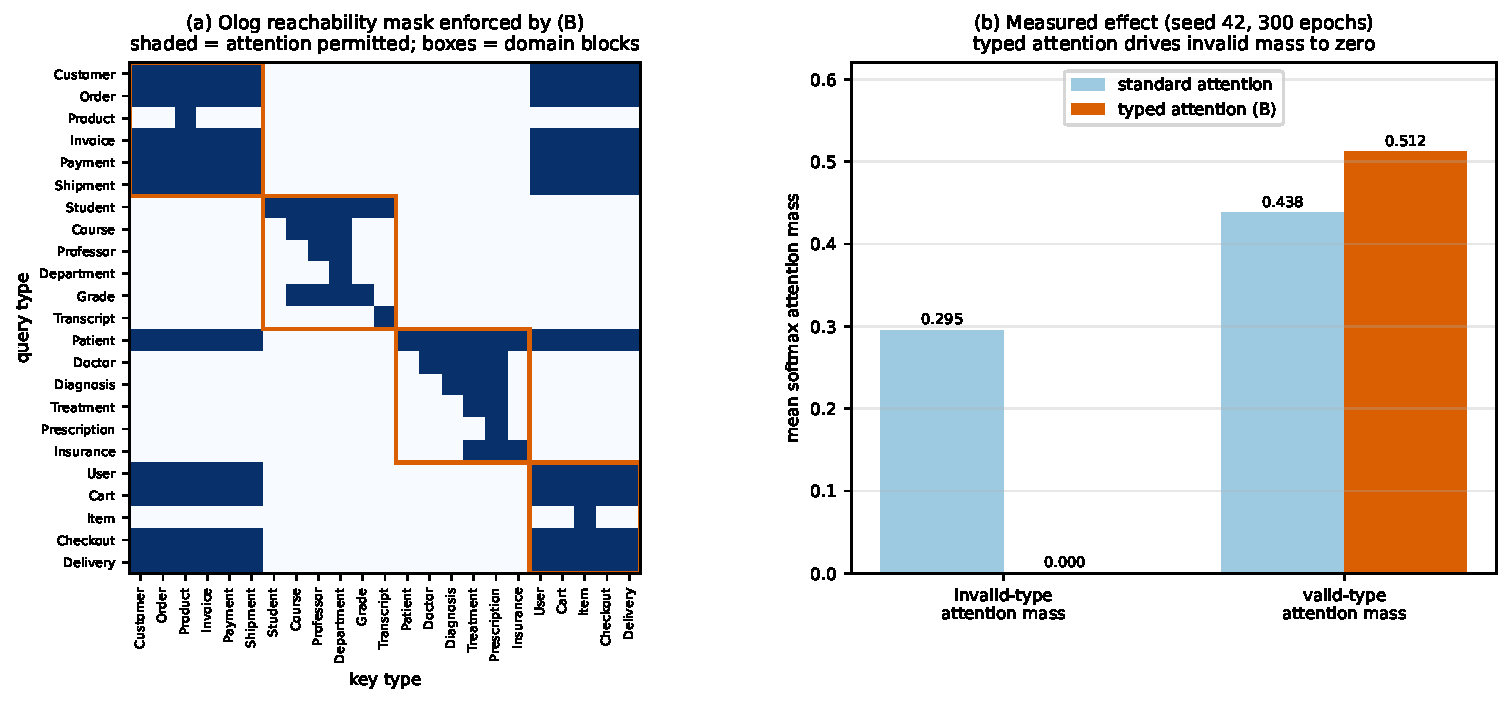
\includegraphics[width=\linewidth]{figures/typed_attention.pdf}
\caption{\textbf{Typed attention (B) and the ontology structure it
enforces.} \emph{(a)}~The reachability mask for the 23-type multi-domain
vocabulary: a query token (row) may attend to a key token (column) only
if the key's type is reachable from the query's under the Olog. The mask
is block-structured --- four domain blocks (orange) plus off-block cells
from the explicit Patient$\to$Customer bridge and the \texttt{Payment}
type shared by the business and e-commerce schemas --- so information
flow is confined to type-respecting paths. \emph{(b)}~The measured
effect (seed 42, 300 epochs; the same run as
Table~\ref{tab:attention_ablation_b}): typed attention drives the mean
attention mass on type-invalid key pairs from 0.295 to exactly 0.000 and
reallocates it onto type-valid pairs (0.438$\to$0.512).}
\label{fig:typed_attention}
\end{figure}

Figure~\ref{fig:typed_attention} shows both sides of this result: the
block-structured reachability mask the (B) layer applies (panel a), and
the redistribution of attention mass it produces (panel b).

\paragraph{(B$'$) is necessary but not sufficient for trajectory soundness.}
A sampling-time projection of (B), denoted (B$'$), admits any next label
whose target type is reachable from the current state. Reachability is
the transitive closure of the Olog morphisms: it admits the eventual
destination without requiring each step to correspond to a $\delta_\mathcal{O}$
edge. A trajectory then breaks at the next step.

\begin{table}[t]
\centering
\caption{\textbf{Two-locus type safety, (B$'$) vs (D).} \emph{Trajectory
soundness} is the fraction of generated trajectories that decode to a
valid $\delta_\mathcal{O}$-path through the Olog (higher is better; 100\%
means every emitted trajectory is type-admissible end to end).
\emph{Reach.} is the fraction of ordered type pairs related by
reachability. \emph{GOOD}/\emph{BAD} are well- and mis-aligned synthetic
label priors. (B$'$), the sampling-time projection of typed attention,
gives only a modest lift over the unconstrained baseline (A) on an
acyclic Olog and collapses to within a point of it once a cycle makes
reachability universal --- whereas the (D) constrained decoder stays at
100\% regardless of topology. Numbers from
\texttt{experiment\_loci\_comparison.py} and
\texttt{experiment\_cyclic\_stress.py}, $N{=}1000$ trajectories per cell,
seed 42.}
\label{tab:b_prime_vs_d}
\begin{tabular}{lccccc}
\toprule
Olog topology & Reach. & (A) GOOD & (B$'$) GOOD & (B$'$) BAD & (D) \\
\midrule
Acyclic & 34.7\% & 48.1\% & 65.0\% & 3.9\% & 100\% \\
Cyclic ($\Delta$Olog: Delivery$\!\to\!$Customer) & 100\% & 6.9\% & 8.0\% & 0.0\% & 100\% \\
\bottomrule
\end{tabular}
\end{table}

This empirically realizes the architectural prediction of
\S\ref{sec:method:two_loci}: (B) restricts information flow inside the
model but does not constrain output emission, so a (B)-only system can
still emit trajectories that violate $\delta_\mathcal{O}$. Under cyclic
Ologs the reachability mask degrades to no-constraint while (D) is
robust to topology.

\paragraph{(D) constrained decoder closes the gap.}
With the (D) constrained decoder enabled, trajectory soundness reaches
100\% on the same harness, including under cyclic Olog stress
(Table~\ref{tab:b_prime_vs_d}, last column). (D) and (B) are
independent: (B) operates on attention weights inside the model; (D)
operates on output logits at sampling. The composition (B)+(D) is both
information-flow-clean (from B) and trajectory-sound (from D).

\paragraph{Real-attention mask audit.} A structural integration test
runs the production typed-attention layer on a 6-token cyclic-Olog
trajectory window. Of the $36$ ($q,k$) pairs, $6$ are self,
$\mathbf{6}$ correspond to $\delta_\mathcal{O}$-direct edges, and
$\mathbf{24}$ are reachable-only --- a $4{:}1$ leakage ratio of pairs
that (B) admits but (D) blocks. Random-init forward-pass attention mass
distributes as $16.9\%$ self / $16.4\%$ direct-edge / $\mathbf{66.7\%}$
reachable-only / $0\%$ unreachable: two-thirds of the attention budget
lands on type-pair categories outside $\delta_\mathcal{O}$. The mask
itself does not push mass toward direct-edge pairs; it allows
everything reachable. This empirically validates the (B$'$) reduction we
used above against the production
$\texttt{OntologicalAttention}$ layer.

\subsection{C3: Topology Contrast}

We compute the first Betti number $b_1 = m - n + b_0$ of the raw entity multigraph as a graph-topological consistency score, distinct from the sheaf-theoretic $H^1$ of C1 (see Appendix~\ref{app:sheaf} for the distinction).
Table~\ref{tab:topology} shows WN18RR's hypernym tree scores 0.633 versus 0.292 for Freebase, correctly reflecting that WordNet encodes a near-tree ontology while Freebase encodes a dense multi-relational web.

\begin{table}[t]
\centering
\caption{\textbf{Topology contrast (C3).} The \emph{consistency} score is
derived from the first Betti number $b_1 = m - n + b_0$ of the entity
multigraph ($n$ entities, $m$ edges, $b_0$ connected components): a
low $b_1$ relative to graph size means few independent cycles, i.e.\ a
near-tree structure. WordNet's hypernym hierarchy scores 0.633 and is
fully connected ($b_0{=}1$); Freebase's multi-relational web scores
0.292 and fragments into 8 components. The score correctly separates a
tree-shaped ontology from a dense relational one --- a distinction
accuracy benchmarks discard. Computed in $O(n+m)$; this is
graph-topological consistency, distinct from the sheaf-theoretic $H^1$
of C1 (Appendix~\ref{app:sheaf}).}
\label{tab:topology}
\begin{tabular}{lrrrr}
\toprule
Dataset & Entities & Edges & $b_0$ & Consistency \\
\midrule
FB15K-237 & 12{,}734 & 43{,}601 & 8 & 0.292 \\
WN18RR & 39{,}621 & 62{,}547 & 1 & \textbf{0.633} \\
\bottomrule
\end{tabular}
\end{table}

\subsection{Link Prediction (Reference)}

For completeness we report link-prediction accuracy on FB15K-237 alongside standard baselines.
Our HDC/Sheaf model reaches MRR~0.346 and Hits@10~0.524, on par with KG-BERT-class baselines, while adding the structural guarantees (sheaf $H^1$ inconsistency signal, typed derivation per prediction) that those baselines do not provide.
We do not claim state-of-the-art link prediction.

\begin{table}[t]
\centering
\caption{\textbf{Link prediction on FB15K-237, for reference.} MRR is the
mean reciprocal rank of the correct tail entity; Hits@$k$ is the fraction
of test queries whose correct tail is ranked in the top $k$ (both higher
is better). The HDC/Sheaf model is on par with KG-BERT-class baselines on
raw retrieval, confirming that the structural layer (Tables
\ref{tab:conflicts}--\ref{tab:topology}) is not bought at the cost of
accuracy. We do not claim state-of-the-art link prediction; the
contribution is the interpretability and consistency guarantees the
baselines lack.}
\label{tab:link_prediction}
\begin{tabular}{lcccc}
\toprule
Model & MRR & Hits@1 & Hits@3 & Hits@10 \\
\midrule
ConvE~\cite{conve2018} (reported) & 0.325 & 0.237 & 0.356 & 0.501 \\
RotatE~\cite{rotate2019} (reported) & 0.338 & 0.241 & 0.375 & 0.533 \\
KGT5~\cite{saxena2022sequence} (reported) & 0.300 & 0.221 & --- & 0.461 \\
SimKGC~\cite{wang2022simkgc} (reported) & 0.336 & 0.249 & 0.362 & 0.511 \\
HDC/Sheaf (ours) & \textbf{0.346} & 0.242 & 0.425 & \textbf{0.524} \\
\bottomrule
\end{tabular}
\end{table}

\subsection{Ablations}

The topology comparison in Table~\ref{tab:b_prime_vs_d} (acyclic vs.\
cyclic Olog) is the primary structural ablation: it confirms the
architectural prediction that (B) degrades under cycles while (D) does
not. The HDC embedding-dimension sweep (1024 / 2048 / 4096 / 8192) with
learning-rate and diffusion-time sensitivity is reported in
Appendix~\ref{app:sweep}. One ablation remains genuinely open --- the
synthetic (B$'$) proxy versus a real-attention forward pass with a
trained label head --- and the four-cell (A / B / D / B+D) ablation that
would disentangle the individual contributions of typed attention and
constrained decoding is scoped as future work (Appendix~\ref{app:b_vs_d}).

\subsection{Limitations}
\begin{itemize}
\item \textbf{Single-scale framing.} The present paper deliberately reports
two independent topological measurements at different scales: cellular
sheaf $H^1$ on the type graph (C1, $\leq 100$ nodes) and graph $b_1$ on
the entity graph (C3, $\sim 10^4$ entities). They answer different
questions and are not connected by a sheaf morphism in this work. A
unified multi-scale persistent-sheaf-cohomology framework is the natural
generalization (\S\ref{sec:conclusion}) but is left to future work.
\item \textbf{(B) accuracy trade-off measured without (D).}
Typed attention~(B) reduces test accuracy by 1.8pp ($0.474 \to 0.457$)
in exchange for full elimination of invalid attention weight
($0.295 \to 0.000$). The measurement is taken with (B) alone, no (D)
decoder. Whether (B)+(D) jointly preserves accuracy as well as (D)
alone is an open empirical question; we conjecture (B) provides a
training-time representation prior that (D) does not, but disentangling
the two effects requires a four-cell ablation (A / B / D / B+D) we did
not run within this paper's scope (see \S\ref{sec:conclusion} and
Appendix~\ref{app:b_vs_d}).
\item \textbf{Single seed on attention ablation.} Table~\ref{tab:attention_ablation_b}
and Figure~\ref{fig:typed_attention}(b) are reported at a single seed
(42); a multi-seed re-run is pending.
\item \textbf{Sparse sheaf cohomology.} Query-time diffusion uses sparse
Krylov methods, but the cohomology computation itself remains dense.
A sparse-Krylov sheaf-cohomology algorithm is left to future work.
\item \textbf{Cyclic Olog stress test.} Reported in Appendix~\ref{app:cyclic};
under a cyclic Olog the (B$'$) reachability mask collapses to within a
point of the unconstrained baseline as reachability becomes universal,
confirming the predicted topological limit.
\end{itemize}
